\documentclass{article}
\usepackage[utf8]{inputenc}
\usepackage{gensymb}
\usepackage{amsmath,physics}
\usepackage{braket}
\usepackage{siunitx}
\usepackage{graphicx}
\usepackage{hyperref}
\usepackage{cleveref}
\usepackage{float}
\usepackage[margin=1in]{geometry}
\usepackage[maxbibnames=99]{biblatex}
\bibliography{mybib}
\setcounter{secnumdepth}{0}
\hypersetup{
    colorlinks,
    citecolor=black,
    filecolor=black,
    linkcolor=black,
    urlcolor=black
}


\title{Literature Review Template}
\author{Cole Lord-May}
\date{}

\begin{document}

\maketitle
\tableofcontents
\newpage


\def \sect {Mahrt1987}
\section{\citeauthor{\sect} \citeyear{\sect}}
\textbf{\citefield{\sect}{title}\nocite{\sect}}
\subsection*{Summary}
This study also explores means of analyzing aircraft-measured turbulence data. As such, it is also somewhat less directly pertinent, but makes interesting comments on examining periodic, shear-driven turbulence. 
This paper is worth re-reading somewhat often, as it provides good physical insight into the mechanisms responsible for turbulence and what it ``looks like".
\subsection*{Important Figures}
\begin{figure}[ht]
    \centering
    \vspace{-4mm}
    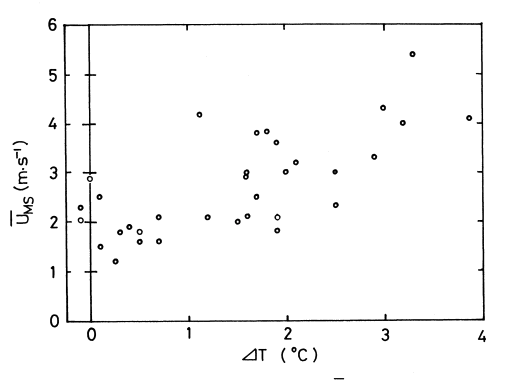
\includegraphics[width=80mm]{\sect/1.png}
    \vspace{-4mm}
    \caption{Illustrations of structure functions given synthetic input data}
    \label{f:mahrt1987_1}
\end{figure}
\begin{figure}[ht]
    \centering
    \vspace{-4mm}
    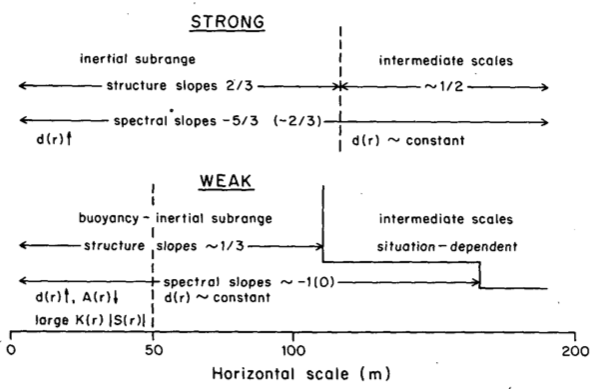
\includegraphics[width=80mm]{\sect/2.png}
    \vspace{-4mm}
    \caption{Scale regimes for weak and strong turbulence. \(d(r)\) is buoyancy length, \(S(r)\) is skewness, and \(S(r)\) is kurtosis.}
    \label{f:mahrt1987_2}
\end{figure}
\subsection*{Questions and Comments}
\begin{itemize}
\item The structure functions of various orders seem highly applicable to studying turbulence (as has been done many times before) \cref{f:mahrt1987_1} shows the value of using a structure function instead of data or spectra. The structure function extracts the general shape of the data (the integral of the data) but smooths fluctuations and avoids the many frequencies in spectra. These might be useful inputs into PCA!
\item They define the buoyancy length (as a measure of stratification strength) as \(D_{ww}/\left(g/\Theta_0D_{\theta\theta}^{1/2}\right)\). This might be a more general measure than $z/L$. I haven't seen this explored much as a classification of inversion, so it would be worth investigating. It doesn't require computation of vertical gradients, and is not tied to horizontal scales.
\item \cref{f:mahrt1987_2} is a very visually clear separation of turbulence. They first classify turbulence into weak and strong, and then draw out the horizontal scales over which different spectral slopes exist. Being able to distinguish turbulence in such a clear way would be very illuminating to our turbulence on the glacier slope.
\item The cospectructure functions that they introduce allow them to distinguish between bora turbulence and nocturnal boundary layer turbulence. This would be fascinating if we could distinguish between origins of turbulence origins. However, I suspect that below the wind speed max, most of the turbulence would have the same origin.
\item They find that at intermediate scales of turbulence, spectral slopes are influence by turbulence strength and not by mechanics. This suggests that a fairly significant key of the turbulence-in-stratified-fluids puzzles isn't being properly accounted for (as this should never be the case if you truly have critical phenomena).
\end{itemize}
\newpage



\def \sect {Ohata1989}
\section{\citeauthor{\sect} \citeyear{\sect}}
\textbf{\citefield{\sect}{title}\nocite{\sect}}
\subsection*{Summary}
Observations made on the 40~km-long San Rafael Glacier in the Patagonia Northern Icefield from 1983-1984. Data was collected from four observation sites on the ground and two observation sites on the glacier. 
In addition to higher-frequency measurements of mean temperature, mean wind speed, and temperature inversion at a fixed height, 19 wind profile measurement were made at random times throughout the day. 
Glacier wind height \(h\) is measured as the maximum height at which predominant wind direction is still down-slope, or when wind speed decreases below \SI{1}{\m\per\s} -- whichever is lower. The measured thickness of the glacial wind varied between \SI{30}{\m} and \SI{120}{\m}. 
They measured that the height of the wind maximum \(h_m\) was typically half of \(h\), \(h_m/h\approx0.5\). This is substantially higher than Prandtl's model, which is attributed to a higher surface roughness. They concluded that even with a low lapse rate, (\(\Delta T<\SI{1}{\celsius}\) over \SI{100}{\m}), glacier winds are still the predominant daytime feature, occurring \(~80-90\%\) of the time. 
There appears to be a consistent fluctuation in mean wind speed, with a nighttime period of 3 hours and a daytime period of 1-2 hours.
\subsection*{Important Figures}
\begin{figure}[ht]
    \centering
    \vspace{-4mm}
    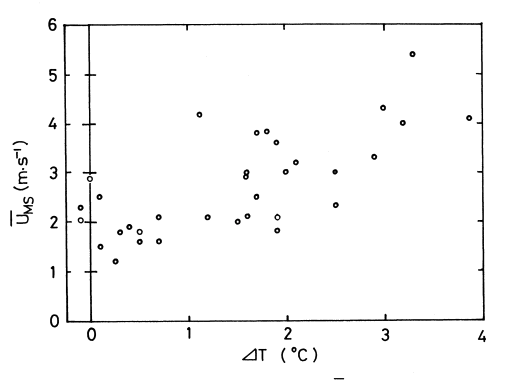
\includegraphics[width=80mm]{\sect/1.png}
    \vspace{-4mm}
    \caption{Comparison of observed temperature inversion strength \(\Delta T\) and wind speed -- confirming that high wind speeds are driven by strong temperature inversions}
    \label{f:down}
\end{figure}
\newpage






\printbibliography
% \bibliographystyle{apalike}
% \bibliography{prop}

\end{document}
